%!TEX root = ../report.tex

\begin{document}
    \chapter{State of the Art}
	This chapter aims to explain the state-of-the-art uncertainty estimation methods considered for this research work. 
	\section{Dropout as Bayesian Approximation}
	The method proposed by Gal {\etal} [\cite{gal2016dropout}] estimates model uncertainty in Neural Net models using Dropout [\cite{srivastava2014dropout}] which is a commonly used regularization technique. The work proves the equivalence between a Dropout applied Neural Network model and an approximated Deep Gaussian process model and establishes Dropout as a means to approximate the posterior predictive distribution. The absence of any need to make changes to the optimization process for integrating this method to a Neural Network model can be considered as one of its unique features. The technique applies to Neural Nets meant for both classification and regression tasks. 
	
	In order to obtain model uncertainty using this method in practice, dropout is enabled during the test-time and a given input is passed through the Neural Network a number of times equal to the pre-defined Monte-Carlo sample count hyper-parameter. The sample mean and variance of multiple stochastic forward passes correspond to the final model output and model variance respectively. 
	
	Though this method forms the basis of a few uncertainty estimation methods like [\cite{loquercio2020a}], the need for multiple stochastic forward passes makes it computationally expensive and unsuited for real-time applications.
	
	\section{Deep Ensembles}
	  Deep Ensembles [\cite{lakshminarayanan2017simple}] is a non-Bayesian approach to estimate predictive uncertainty by using outputs from an ensemble of Neural Networks. The work by LakshmiNarayanan {\etal}  also proposes the idea of leveraging adversarial perturbations generated using the Fast Gradient SignMethod(FGSM)[\cite{goodfellow2015explaining}], to smoothen predictive distributions.
	  
	  Authors show advantages of using Deep Ensembles over the base-line approach proposed by Gal {\etal} [\cite{gal2016dropout}].The ability to report of high uncertainty estimates for Out-Of-Distribution and adversarial samples is claimed and proved by evaluating the method on a number of datasets for both regression and classification tasks. The work can be considered as one of the first frequentist approaches to estimate predictive uncertainty in Neural Networks.
	  
	  With an increase in the number of member networks in an ensemble, the neural net model size increases as well. Therefore, the method is not suitable for very deep network architectures. Also, the need for diversity amongst ensemble members has a significant impact on the quality of estimated uncertainty.  
	\section{Light-weight probabilistic deep networks}
	 Lightweight Probabilistic Deep Networks [\cite{gast2018lightweight}] by Gast {\etal} enables conversion of a deterministic Neural Network to its probabilistic equivalent which is capable of propagating and outputting parameters of the predictive distribution, in turn uncertainty linked to it. The conversion is achieved in two steps: 
	 \begin{itemize}
	 \item Introducing a probabilistic output layer that produces moments of the predictive distribution as its outputs.
	 \item Replacing intermediate activations with their probabilistic equivalents. Assumed Density Filtering(ADF)(explained in \ref{sec_adf}) a form of Expectation Propagation is used to achieve it. 
	 \end{itemize}
	 
	 The need for minor architectural changes and no change in the optimization process is a key feature of this method. The method does not represent weights probabilistically, which results in over-confident predictions.
	  
	\section{Prior Networks}
	Malinin \etal [\cite{malinin2018predictive}] proposed a technique to estimate predictive uncertainties in Neural Nets for classification, by parameterizing a prior distribution over the predictive distribution. The work uses Dirichlet distribution as the higher-order(prior) distribution over predictive categorical distributions, due to existence of  conjugate prior relationship between the pair which makes the posterior analytically tractable. In this way, the variances(uncertainties) around parameters of the categorical distribution are modeled. Parameters of the higher-order distribution are included as a part of the loss function which gets optimized.
	
	 Prior Networks can be considered as one of the earliest works when it comes to learning how to model uncertainty from the given training data.Another important contribution of this work is that the method separates out the uncertainty that arises due to mismatch between training and test data distributions as \enquote{distributional uncertainty}. Authors claim the work to outperform other uncertainty estimation methods when it comes to reporting misclassification and Out-Of-Distribution(OOD) input samples.
	
	
	The proposed method is defined for classification setup and therefore cannot be used in regression nets. Also, the work lacks strong experimental evaluation as its assessed only on toy datasets with two other uncertainty estimation methods.
	
	\section{Choice of methods for this research work}
	The methods listed so far suffer from at least one of the following downsides: increased model inference time, increased model size, under/over estimation of uncertainties , disregard any relationship between components of uncertainty. This research work considers \enquote{A General Framework for Uncertainty Estimation in Deep Learning} [\cite{loquercio2020a}] and \enquote{Deep Evidential Regression}[\cite{amini2020deep}] for benchmarking, based on claims made by their authors that they overcome deficits of other methods, as listed above. The rest of this chapter explains both the methods descriptively.
	\section{A General Framework for Uncertainty Estimation in Deep Learning}\label{general_framework}
	\subsection{Overview}\label{mcdo_adf_overview}
	This work proposes a technique to distinctively estimate data and model uncertainties associated with an output of any Neural Network model.The technique is here after referred to as "MCDO\_ADF", representing the fact that is a combination of two ideas, Monte-Carlo Drop Out(MCDO) and Assumed-Density-Filtering (ADF). MCDO\_ADF treat the  two uncertainty components to be related, which sets it apart from most of other uncertainty estimation methods that treat them to be independent. The method employs Bayesian Belief Networks combined with Monte-Carlo sampling for estimating the model uncertainty and relies on the idea of Assumed Density Filtering for  estimating data uncertainty associated with an output. 
	
	Authors of the MCDO\_ADF technique claim it to be a general framework to estimate uncertainties in Neural Networks. They give following reasons to validate their claim:
	\begin{itemize}
		\item Using this uncertainty estimation method does not require any architectural changes in the target Neural Network.
		\item Applicability of the method to Neural Network models of different tasks.
		\item Absence of any need of make changes in the optimization process.
		\item Ability of the technique to be applied to already trained models.
	\end{itemize}
	
	The upcoming sections of this chapter explain the MCDO\_ADF technique  and also analyze its claimed "generality" by using it in a Resnet8 based Neural Network regression model meant for the application of steering-angle prediction in autonomous cars.(Note: A detailed description of the data set, training and inference procedures of the Neural Network model is available in \ref{chap_methodology}).  
	
	
	\subsection{Integrating MCDO\_ADF with a Neural Network and estimating uncertainties}
	\subsubsection{MCDO\_ADF as an algorithm}
	Estimating uncertainty using the MCDO can be formulated as an algorithm consisting of the following steps:
	\begin{itemize}
		\item Transform the Neural Network of interest to its ADF(Assumed Density Filtering) version.
		\item Collect a predefined number(T) of Monte-Carlo(MC) samples by forwarding inputs and noise variances $(x,v))$ stochastically through the network for T times.
		\item Computation of output predictions and uncertainties  
	\end{itemize}
	\begin{figure}[h]
		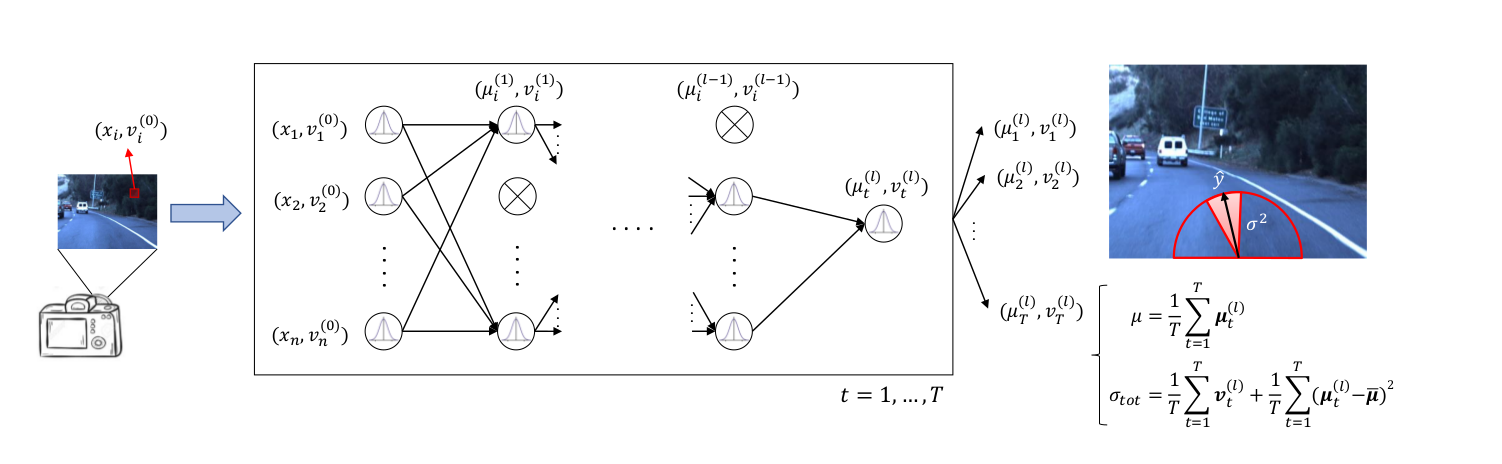
\includegraphics[scale=0.35]{adfmcdo}
		\caption{Illustration of the MCDO\_ADF technique.Here $x_{i}$ denotes the input through the $i^{th}$ unit of a given hidden layer,$x_{i^{(n)}}$ denotes the noise variance input to the ith unit of the nth layer. Circles with crosses inscribed denote the dropped out neurons whereas the ones with the Gaussian distribution symbol denote the active units. T values of $\mu$ and $v$ are collected from T stochastic forward passes. Image source: }
		\label{fig_adf_mcdo}
	\end{figure}
	
	
	
	
	
	\subsubsection{Assumed Density Filtering (ADF)}\label{sec_adf}
	The MCDO\_ADF technique considers sensor noise to be the primary source of data uncertainty in neural network predictions and therefore feeds it to the Neural Network model during the inference. In order to propagate the input data distribution (parameterized by the input as its mean and sensor noise as variance) the technique of ADF is used. Briefly in the context of MCDO\_ADF, ADF replaces every input activation into a probability distribution and also approximates the same using a tractable Gaussian distribution and makes both the mean and noise variance available in the output layer.Following points describe Assume Density Filtering in a more detailed manner:
	\begin{itemize}
		\item Assumed Density Filtering(ADF) is a technique in Bayesian machine learning to approximate intractable and complex distribution with distributions that are easy to handle. In the case of Bayesian Inference, ADF aims to project the true posterior onto a distribution of choice. The exponential family of distributions are a popular choice.
		\item In the case of MCDO\_ADF there is a need to propagate the input data distribution so that the values of its mean and variance (noise variance) are available in the output layer. 
		\item The input data distribution is considered to be Gaussian in nature. Every intermediate layer outputs the transformed version of the input distribution.  However, when it propagates through non-linearities in a Neural Network the resulting distribution need not be essentially another Gaussian. Such a distribution emerging out of non-linear blocks is also conditioned by distribution over activations of the preceeding layers. Therefore, the resulting distribution becomes intractable.
		\item Such intractable and complex distributions are estimated using ADF by:
		\begin{itemize}
			\item Assuming conditional independence between distribution outputted from a given layer with its preceeding layers. 
			\item Approximating the complex distribution with a Gaussian distribution whose pair has the least possible value of Kullback-Leibler divergence(described in \ref{sec_kl_div}). ADF achieves this by matching the first two moments of the distributions.
			\item In practice, this is achieved by optimizing the global variational objective.
		\end{itemize} 
	\end{itemize}
	In practice, every building block of a Neural Network has its corresponding ADF version and therefore during the inference time the entire model has to be transformed to its ADF equivalent. This gives the ability to the Neural Network model to propagate and output distributions which represent data uncertainty.
	\begin{figure}[h]
		\centering
		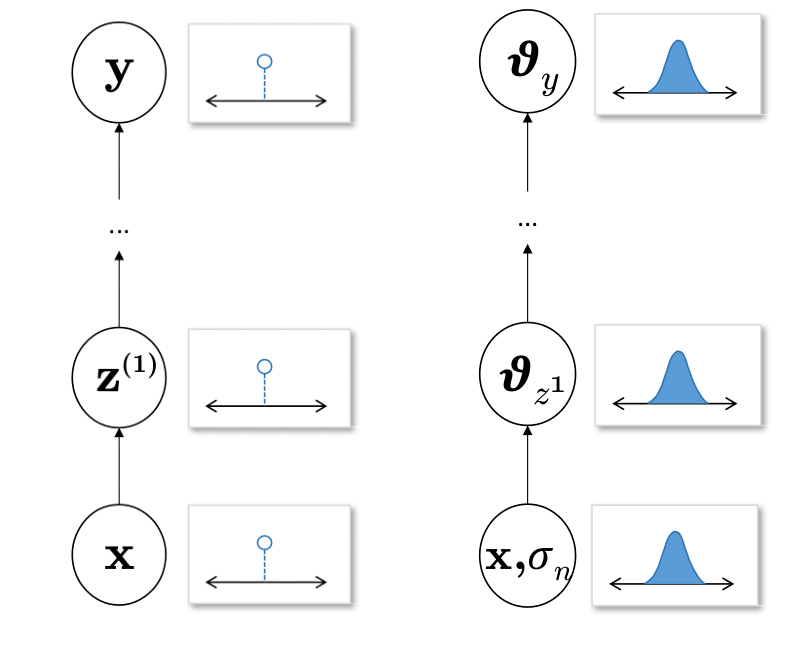
\includegraphics[scale=0.4]{adf_determ}
		\caption{Illustration of forward passes in deterministic and ADF versions of a Neural Network. Here $x$ denotes the input activations,$z^(n)$ denotes activation input to the nth layer,$y$ denotes the output, $\theta_{z^n}$ represents input activation to the nth layer expressed as a probability distribution and $\sigma$ corresponds to the noise variance. Image source: }
	\end{figure}
	
	\subsubsection{Data uncertainty estimation}
	The ADF transformed Neural Network produces two outputs from the final layer: mean ($\mu_{t^{(l)}}$) and variance($v_{t^{(l)}}$ of the propagated distribution, as shown in the figure \ref{fig_adf_mcdo}. The pair of values is outputted for each of the T stochastic forward passes (described in the next paragraph) and the mean of T variance values is considered to be the value of data uncertainty. Likewise, the mean of T predictions is considered to be the model's prediction for the given input.
	\begin{equation}
		prediction = \mu = \frac{1}{T}\sum_{t=1}^{T}\mu_{t^{(l)}}
	\end{equation}	 
	\begin{equation}
		data\_uncertainty = \sigma_{data}=\frac{1}{T}\sum_{t=1}^{T}v_{t^{(l)}}
	\end{equation}
	
	\subsubsection{Monte-Carlo Dropout (MCDO)}
	
	This uncertainty estimation method relies on the idea of Monte-Carlo(MC) sampling to estimate model uncertainty associated any prediction. In practice, MC sampling is achieved by enabling dropout during the test time and obtaining the desired number of samples (T), which are nothing but outputs of the Neural Network model during different forward passes of the input. Enabling dropout introduces stochasticity during those forward passes.
	
	Following points briefly describe the dropout technique in a general context:
	\begin{itemize}
		\item Dropout(\cite{srivastava2014dropout}) is primarily a regularization technique used while training Neural Networks in order to avoid over-fitting.
		\item During dropout certain nodes of a given Neural Network layer are not considered for training. The nodes are ignored with a probability equal to the dropout rate (often denoted by $\textbf{p}$).
		\item Using dropout during training makes Neural Network layers to adapt in such a way that they cope with mistakes made my the prior layers. 
		
	\end{itemize}
	
	In the context of Bayesian inference, the Dropout technique is used to approximate the posterior distribution over weights of a given Neural Network, when the training data and labels are given ($P(W|X,Y))$. The approximation is obtained by applying dropout at the test-time. This makes it possible to obtain multiple predictions for any given input from different architectures resulting from application of dropout to the base Neural Network model. The different architectures obtained along with their weights can be considered as Monte-Carlo(MC) samples from the space of all possible architectures. The number of MC samples to be obtained is a hyper-parameter and denoted by $T$. In another perspective, $T$ equals the number of forward passes through different architectures with different sets of weights $\{W_{1}^t,..,W_{L}^t\}_{t=1}^T$($L$ denotes the number of dropout applied layers in the Neural Network). The first and second moments (mean and variance) of predictions obtained from these stochastic forward passes of given input are utilized to compute model uncertainty(explained in  \ref{adf_mcdo_uncertainty_estimation}). One of the highlights of this technique is that its usage does not require any architectural changes and also can applied to already trained Neural Net models. The hyper-parameters $T$ and $p$ significantly impact the effectiveness of this technique. In the case of $p$ a very high value (close to 1) increases sparsity in nodes and also results in longer convergence-time while a low value eliminates the MC-sampling utility. For our experiment, the value of $p=0.02$ is used. The hyper-parameter $T$ significantly impacts the inference time of a Neural Network model and therefore has to be chosen optimally based on the run-time requirement of the system where the model would be deployed.
	
	\subsubsection{Model uncertainty estimation}
	The MCDO\_ADF technique estimates model uncertainty using predictions generated from the Neural Network model during multiple(T) forward passes, while the dropout is enabled. A given input is processed by the model T times, with a new combination of neurons considered for almost every forward pass. This produces an effect of gathering predictions from an ensemble consisting of T Neural Net models with different architectures. The variance of T gathered predictions is the estimated model uncertainty. In the following equations $\mu_{t^{(l)}}$ signifies the mean output from the ADF transformed version of the Model during $t^{th}$ forward pass.
	
	\begin{equation}
		model\_uncertainty = \sigma_{model} =  \frac{1}{T}\sum_{t=1}^{T}(\mu_{t^{(l)}}-\overline{\mu})^2
	\end{equation}
	\begin{equation} 
		where, \overline{\mu} = \frac{1}{T}\sum_{t=1}^{T}(\mu_{t^{(l)}} 
	\end{equation}
	\subsubsection{Combining ADF and MCDO}
	The MCDO\_ADF method considers a relationship to exist between the two components of uncertainty (data and model). The relationship  is realized in this technique by combining both the ideas of ADF and MCDO. During inference,  
	\begin{itemize}
		\item The given Neural Network model is transformed to its ADF equivalent so that the output layer produces both predictions(mean) and noise variance as the model's final outputs.
		\item For estimating model uncertainty,  dropout is enabled in the ADF transformed version of the original Neural Network following which T MC samples are collected during T stochastic forward passes. It is this application of dropout on the ADF transformed version that produces the "effect of ensembling T ADF Neural Networks" and also considers any relationship between the two uncertainty components.
		\item Combining ADF and MCDO leads to another intuitive realization about the uncertainty components in this setup. Even when a particular input fed to the Neural Net model was observed frequently during training, if corrupted due to sensor noise then it will not only have high values of both data and model uncertainties. 
		
	\end{itemize}
	
	\subsubsection{Total uncertainty}
	The predictive uncertainty is estimated by summing up both its components (data and model) and is given by the following equation.
	\begin{equation}
		predictive\_uncertainty = \sigma_{total} =  \frac{1}{T}\sum_{t=1}^{T}((\mu_{t^{(l)}}-\overline{\mu})^2 + v_{t^{(l)}})
	\end{equation}
	
	
	In summary, both ADF and MCDO techniques approximate probability distributions of data and model with Normal distributions respectively. ADF propagates the input data distribution and approximates them as Gaussians in every Neural Network layer while MCDO approximates the distribution around weights by sampling and forms a Gaussian distribution out of the samples. The variances of these Gaussian distributions are considered to be the uncertainty components and are summed up to yield the predictive uncertainty.
	
	\subsection{Inference procedure}\label{sec_mcdo_adf}
	The MCDO\_ADF method can be applied to already trained deterministic version of the Neural Network models as mentioned in \ref{mcdo_adf_overview}. However, it is also possible to train the Neural Network model of interest with dropout enabled and use the same for inference.
	In order to estimate the predictive uncertainty during inference:
	\begin{itemize}
		\item Every layer of the Neural Network has to replaced with its ADF equivalent so that they are equipped with the ability to propagate data distributions. The implementation of ADF equivalents for most of the Neural Network building blocks is available in the Github repository of \cite{gast2018lightweight}.
		\item The value of noise variance (a constant value) obtained from the sensor's data sheet is fed along with the input data to the ADF transformed input layer of the network. During propagation through intermediate layers, it is ensured that at least a minimum value of variance is propagated. In the case of experiment described in the next chapter, a minimum value of 0.001 is used.
		\item Every input along with the noise variance undergoes T stochastic forward passes through the network to generate T predictions.  
	\end{itemize}
	The experiment described in the next chapter discusses more on practical aspects of this technique.    
	\subsection{Downsides}
	\begin{itemize}
		\item The need for multiple (T) forward passes to obtain MC samples is computationally expensive and cannot be afforded in the case of real-time systems.While there is an option to reduce the value of T, it increases the difference between approximated and underlying distribution over weights of the model, thereby affecting the method's performance. 
		\item The method considers sensor noise to be the only source of data uncertainty. Also, it treats the noise to be additive Gaussian in nature. However, sensor noise is just one of the factors contributing to data uncertainty. For instance, in the case of image data, usage of a lossy compression technique can also contribute to its noise. Also, it is possible for a given sensor to produce data whose noise levels differ. As it is impossible to consider and model every possible noise source, it is important for an uncertainty estimation method to learn to differentiate noise and useful information from given data.
		\item The authors of MCDO\_ADF quote its ability to be applied to already trained models as one of the key reasons for its generality. However, retraining a Neural Network model is something feasible in most of the cases.
		\item As hyper parameters such as drop-out rate($p$), number of MC samples(T) and noise variance have a major role to play in this technique, it adds to the responsibilities of the practitioner to optimally choose them based on the problem at hand.
	\end{itemize}    
	
	\section{Deep Evidential Regression}\label{der}
	
	\subsection{Overview}\label{sec_overview_der}  
	Deep Evidential Regression proposes a method (hereafter referred to as "DER") to estimate predictive uncertainty primarily in Neural Networks for regression, by simultaneously learning a hierarchy of distributions. The learned hierarchy consists of two levels of distributions: 1. A lower level Gaussian distribution over data, with parameters (mean $\mu$ and variance $\sigma^2$) 2. A higher level(also called Evidential) Normal-Inverse Gamma distribution over the parameters of the lower level distribution. In the perspective of the Bayesian Inference, the higher-order distribution can be taken as a prior over the the lower-order distribution which is obtained by evaluating likelihood of known data points for a particular choice of $\mu$ and $\sigma^2$. The evidential distribution evaluated at any particular instance(a combination of $\mu$ and $\sigma^2$  ), provides the subjective belief mass of the corresponding lower-order distribution there. This subjective belief mass is also called as "evidence". Lack of evidence means existence of uncertainty and therefore the value of evidence is used to quantify predictive uncertainty. 
	
	In order to put the above mentioned ideas into practice, DER provides a loss function whose objectives are to:
	\begin{itemize}
		\item Fit the training data to the evidential model.
		\item Learn the evidential prior which would provide uncertainty estimates during inference.
		\item In simple words, to learn the parameters of the higher-order evidential distribution.    
	\end{itemize} 
	The upcoming sections of this chapter explain the method in a detailed manner.
	
	\subsection{Conjugate priors}
	Let us consider a learning problem where Random Variables(RV) $\Theta$ and Y represent model parameters and data respectively. Assuming that RVs are jointly distributed and applying Bayes Rule to determine the probability distribution of $\Theta$ given Y,
	\begin{equation*}
		P(\Theta|Y) = \frac{P(Y|\Theta)P(\Theta)}{P(Y)}
	\end{equation*}
	The equation can be expressed in words as follows:
	\begin{equation*}
		\text{Posterior distribution of $\Theta$ given Y}=\frac{\text{Likelihood of Y given $\Theta$ }.\text{ Prior over $\Theta$}}{\text{Marginal Likelihood of Y}}
	\end{equation*}
	During inference, for a particular choice of functions to represent the likelihood distribution, the nature of prior distribution function matches the nature of posterior distribution function. For example, if a normal distribution with unknown mean and
	variance is used to represent the likelihood distribution and if a Normal-Inverse Gamma distribution(NIG)(described in the next subsection) is used to represent the prior distribution then nature of posterior probability distribution is also observed to be Normal-Inverse Gamma in nature. This can be briefly written as "Normal-Inverse Gamma distribution is the conjugate prior for Normal distribution in likelihood".
	Conjugate priors help to reduce computations involved in determining the $P(\Theta|Y )$ value every time during the process of determining optimal set of parameters. Beta, Gamma and Normal distributions are favorite choices for priors as they act as conjugate priors for different likelihood distribution functions. In the context of DER, the conjugate prior relationship between distributions is used to introduce a hierarchy between the them to probablistically model the likelihood distribution. 
	\subsubsection{Distribution hierarchy}
	Let us assume using a Normal distribution $\mathcal{N}(\mu,\sigma^2)$ to model a set of data points $x_1,x_2,..,x_i$."When a probability distribution A is used to model the given set of data, the uncertainty in the fit is described by probability distribution/s B over parameters of A". This means defining probability distributions over the set of parameters $\mu,\sigma^2$ helps in describing uncertainty in the model fit.
	 
	The probability distribution of $\mu$ is modeled by a normal distribution due to its Gaussian nature and the fact that $\mu \in \mathbb{R}$. On the other hand, a Gamma distribution($\Gamma(\alpha,\beta)$) is used to model the probability distribution of $\sigma^2$ owing to its strictly positive nature. The following figure illustrates hierarchical relationship between distributions under consideration, where $(\mu_0,\sigma^{2}_0),(\alpha,\beta)$ represent the parameters of the higher-order Normal and Gamma distributions respectively.
	
	\begin{figure}[h]
		\centering
		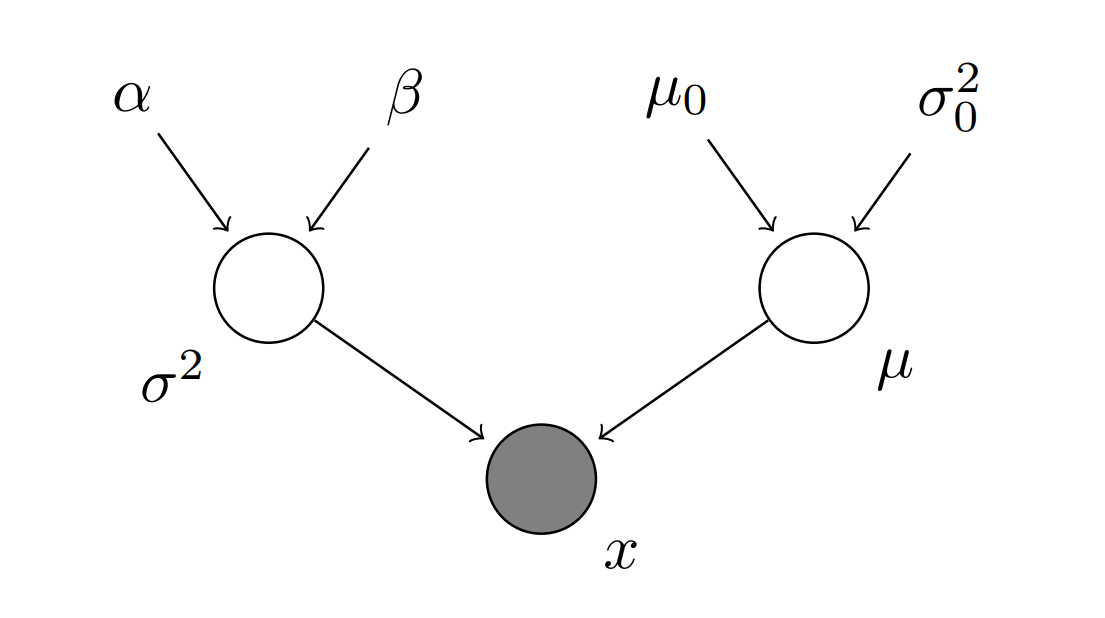
\includegraphics[scale=0.3]{nig_norm_hierarchy}
		\caption{Hierarchy in distribution parameters.Image source: }
		\label{fig_nig_norm_hierarchy}
	\end{figure}
	
	Alternatively, a Normal-Inverse-Gamma distribution (often represented as NIG($\alpha$,$\beta$,$\gamma$,$\lambda$)) can be used to model the probability distribution of $\mu$ and $\sigma^2$ jointly. DER uses the distribution to realize its objectives. Significance of NIG's parameters is explained under the next section.
	
	\subsection{Evidential distribution}\label{sec_evidential_dist}
	\subsubsection{From the perspective of Bayesian inference}\label{sec_persp_bayes}
	Let us consider a regression problem with an available dataset $D$ with N pairs of data labels and targets represented by $(x_1,y_1),..,(x_N,y_N)$. The DER method assumes that the targets are  drawn independent and identically from a Gaussian distribution with unknown mean and variance represented by $\mu$ and $\sigma^2$ respectively.
	\begin{equation}
		(y_1,..,y_N) \sim \mathcal{N}(\mu,\sigma^2)
	\end{equation} 
	
	The parameters $\mu$ and $\sigma^2$ are considered to be random variables that follow Gaussian and Inverse-Gamma distributions respectively.
	
	\begin{align}
		\mu &\sim \mathcal{N}(\gamma,\sigma^2\lambda^{-1})\\
		\sigma^2 &\sim \Gamma^{-1}(\alpha,\beta)
	\end{align}
	where $\alpha, \beta, \gamma, \lambda$ denote parameters of the higher-order Normal Inverse Gamma (NIG) distribution. Let $\theta = (\mu,\sigma^2)$ denote the parameters of one instance of Gaussian distribution generating targets $y_{i}$  and $m = (\alpha, \beta, \gamma, \lambda)$ denote the set of NIG distribution parameters.
	
	
	We are interested to model the distribution around $\theta$. Applying Bayes Rule, we get
	\begin{equation}\label{eqn_bayes_der}
		P(\theta|m) = \frac{P(m|\theta)P(\theta)}{P(m)},
	\end{equation}
	
	\begin{equation*}{}
		\text{posterior. dist. over $\theta$ for the given value of m} = \frac{\text{likelihood of m evaluated at the given value of $\theta$ x prior over $\theta$}}{\text{likelihood of m evaluated at all possible values of $\theta$}}
	\end{equation*}
	
	Here, the prior over $\theta$ is a NIG distribution and the likelihood function is Gaussian in nature. Therefore, the posterior takes the form of an NIG distribution expressed as follows:
	\begin{equation}
		P(\mu,\sigma^2\mid\gamma,\lambda,\alpha,\beta) =  \frac {\sqrt{\lambda}} {\sigma\sqrt{2\pi} } \, \frac{\beta^\alpha}{\Gamma(\alpha)} \, \left( \frac{1}{\sigma^2} \right)^{\alpha + 1}   \exp \left( -\frac { 2\beta + \lambda(\gamma - \mu)^2} {2\sigma^2}  \right)
	\end{equation} 

	\subsubsection{Significance of NIG parameters}\label{sec_nig_param}
	$\gamma$  and $\alpha$ are shape and location parameters of NIG distribution respectively. $\beta$ refers to the inverse-scale (rate) parameter. This means that spread of the distribution is inversely related to $\beta$. There is a relationship that exists between parameters of the NIG distribution. $\gamma$ can be interpreted as the sample mean of $\lambda$ virtual observations, determining NIG's location. On the other hand, spread of the NIG distribution  can be considered to have calculated from 2$\alpha$ virtual observations whose sample mean equals $\gamma$ and their squared deviations summing to 2$\beta$. DER considers the count of virtual observations as evidence($\phi$) in support of the data sample at hand.   
	\begin{equation}\label{eqn_evidence}
		\phi = \lambda + 2\alpha
	\end{equation}
	\begin{figure}[h]
		\centering
		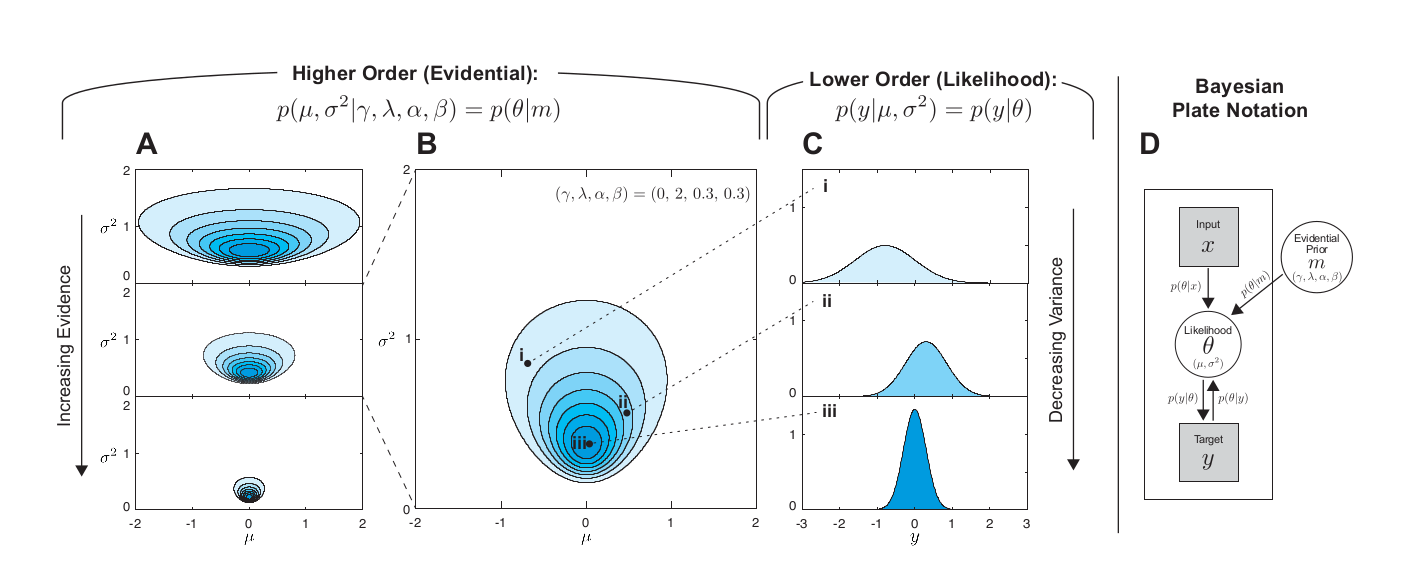
\includegraphics[scale=0.37]{nig}
		\caption{Realizations of the NIG distribution.  Image source: }
		\label{fig_nig_realization}
	\end{figure}
	Figure \ref{fig_nig_realization} illustrates the impact of increase in evidence on the shape and spread of the NIG distribution (column \textbf{A}) and various realizations of the lower-order likelihood distribution (column \textbf{C}) from a given instance of NIG distribution(column \textbf{B}). Following are some of the key insights that can be obtained from the illustration:
	\begin{itemize}
		\item With increase in evidence (as expressed in \ref{eqn_evidence}) the belief mass increasingly concentrates around a specific value pair of $\mu$ and $\sigma^2$ in the column \textbf{A} meaning a reduction in uncertainty.
		\item Column \textbf{B} illustrates the evidential distribution  centered around a particular value pair of $\mu$ and $\sigma^2$. This intuitively means that every point on the distribution corresponds to parameters of a possible likelihood distribution. 
		\item  Sampling the higher order distribution at various locations yield likelihood distributions of varying levels of evidence associated with them. Column \textbf{C} in the illustration shows such realizations. Darker the blue shade used to represent a likelihood-distribution, higher the evidence level associated with it.  
	\end{itemize}
	\subsection{Evidential learning objectives}\label{sec_evi_learning_objectives}
	As described in the overview(\ref{sec_overview_der}), the objectives of DER are two fold: 1. Maximize the model fit and 2. Minimize the evidence measure in an event of error. The method realizes these objectives in form of a loss function/s(two forms) which is integrated to the Neural Network of choice and optimized during training. 
	
	\subsubsection{Maximizing the model fit}
	This objective of DER focuses on learning the underlying patterns in the data and also increasing the belief mass/evidence in favor of right predictions.
	
	Rewriting the equation \ref{eqn_bayes_der}
	\begin{equation*}
		P(\theta|m) = \frac{P(m|\theta)P(\theta)}{P(m)}
	\end{equation*}
	
	Let us assume that we observe our target $y_i$ which when added to the above equation yields,
	
	\begin{equation}
		P(\theta|y_i,m) = \frac{P(y_i|\theta,m)P(\theta|m)}{P(y_i|m)}
	\end{equation}
	
	Before interpreting the above equation it is important to recollect the fact that in Bayesian Inference every Random Variable(RV) involved is considered to be jointly distributed. In the case of above equation, Random Variables $Y$,$\Theta$ and $M$ corresponding to $y_i$, $\theta$ and $m$ are jointly distributed.
	
	In the above equation, we determine the probability distribution around $\theta$ when it is conditioned under specific values of  $y_i$ and $m$. The two terms in the numerator denote likelihood and prior as described in \ref{sec_persp_bayes}. The denominator term is termed as "marginal likelihood" or "evidence" in Bayesian inference, as it yields the total probability mass  of $Y=y_i$ for all possible realizations of $\theta$ in the model parameterized by $m$. The evidence term is also important to normalize the likelihood so that it represents a probability measure. Column $D$ of the figure \ref{fig_nig_realization} illustrates Bayesian inference in DER.
	The marginal likelihood term can be represented mathematically as follows:
	\begin{align}
		P(y_i|m) &= \int_{\theta}P(y_i|\theta,m)P(\theta|m)d\theta	\\
		P(y_i|m) &=\int_{\sigma^2=0}^{\infty}\int_{\mu=-\infty}^{\infty}P(y_i|\mu,\sigma^2)P(\mu,\sigma^2|m)d\mu d\sigma^2
	\end{align}
	
	The proposed loss function aims to determine the set of parameters m which maximizes the term $P(y_i|m)$(evidence) for the given target $y_i$. Similar to Maximum Likelihood Estimation, the objective of maximization of marginal likelihood is re-framed as minimization of negative log of marginal-likelihood(NLL) for computational convenience.
	The loss function is expressed as:
	\begin{align}
		\mathcal{L}_i^{NLL}(w)&=-logP(y_i|m)\\
		\mathcal{L}_i^{NLL}(w)&= -log(2^{0.5+\alpha}\beta^\alpha\sqrt{\frac{\lambda}{2\pi(1+\lambda)}}(2\beta+\frac{\lambda(\gamma-y_i)^2}{1+\lambda})^{-0.5-\alpha})
	\end{align}
	Alternative to the usual way of minimizing Negative log likelihood the author proposes yet another form for the loss function which minimizes sum-of-squared errors between the prior and data sampled from the likelihood function. Following is the expression for the Sum Of Squared errors(SOS) version of the loss function:
	\begin{equation}
		\mathcal{L}_i^{SOS}(w)=(\frac{\Gamma(\alpha-0.5)}{4\Gamma(\alpha)\lambda\sqrt{\beta}})(2\beta(1+\lambda)+(2\alpha-1)\lambda(y_i-\gamma)^2)
	\end{equation}
	The author claims the SOS version of loss function to be relatively stable while training and also to perform better than the other during evaluation. The portion of loss function $\mathcal{L}$ described in this section only achieves the "model fitting" objective of DER. 
	
	\subsubsection{Minimizing evidence on errors}
	The second objective of DER aims to minimize the evidence measure or to inflate uncertainty in the absence of training data. DER expresses this objective by adding a regularizer term to the loss function which penalizes the loss function in an event of its prediction deviating from the ground truth label. The penalty is scaled by evidence which expressed as sum of virtual observations as described in \ref{eqn_evidence}. Following is the expression for the regularizer term,
	\begin{equation}
		\mathcal{L}_{i}^R(w) = \left\| {y_i - \gamma}\right\|.(2\alpha+\lambda)
	\end{equation}
	Here p refers to the order of norm used to represent the difference between the ground truth label $y_i$ and predicted mean $\gamma$. Author uses the value of p=1 claiming it to be stable during the training process.
	
	Putting both its objectives together the evidential loss function can be expressed as:
	\begin{equation}
		\mathcal{L}_i(w) = \mathcal{L}_i^{SOS}(w) + \mathcal{L}_{i}^R(w)
	\end{equation}
	
	\subsection{Estimating uncertainty}
	Epistemic uncertainty which quantifies the model's inherent lack of knowledge associated with an output can be expressed as the variance around its predictions.
	\begin{equation}\label{eqn_der_epi}
		Var(\mu) = \frac{\beta}{(\alpha - 1)\lambda}
	\end{equation}
	The $\lambda$ term in the denominator refers to the number of virtual observations.
	Aleatoric uncertainty can be computed with the following expression:
	\begin{equation}\label{eqn_der_ale}
		\centering
		\mathbb{E}[\sigma^2]=\frac{\beta}{\alpha -1}
	\end{equation}
	From equations \ref{eqn_der_ale} and \ref{eqn_der_epi} both components of uncertainty can be related as follows:
	\begin{equation}
		\centering
		epistemic\_uncertainty = \frac{aleatoric\_uncertainty}{\lambda}
	\end{equation}
	This means that the epistemic uncertainty component is the mean of aleatoric uncertainty over $\lambda$ virtual observations.
	
	Predictive uncertainty can be evaluated as the sum of epistemic and aleatoric uncertainty components.
	\begin{equation}
		predictive\_uncertainty= aleatoric\_uncertainty + epistemic\_uncertainty
	\end{equation}
	\text{From eqns \ref{eqn_der_ale} and \ref{eqn_der_epi} predictive uncertainty can be computed as follows:}\\
	\begin{equation}
		predictive\_uncertainty= \frac{\beta}{\alpha -1} + \frac{\beta}{(\alpha - 1)\lambda}
	\end{equation}
	\text{After simplification,}
	\begin{equation}
		predictive\_uncertainty = \frac{\beta(1+\lambda)}{(a-1)\lambda}
	\end{equation}
\end{document}
